\documentclass[letterpaper,onecolumn,titlepage]{Ythesis}

\usepackage[utf8]{inputenc}
\usepackage{tikz}
\usetikzlibrary{mindmap}

\usepackage{graphicx}
\graphicspath{{sections/figs/}{.figs/}}

\usepackage[backend=bibtex, style=numeric-comp]{biblatex}
\bibliography{glasslab_viz}

\usepackage{array,multirow,graphicx}
\usepackage{subcaption}
\usepackage{subfiles}
\usepackage{url}
\usepackage{amsmath}


\title{Visualizing Conditional Dependencies}
\author{Hannah Aizenman}
\committee{Dr. Michael Grossberg(Advisor), Dr. Robert Haralick, Dr. Lev Manovich, Dr. Huy Vo}
\submitted{}
\abstract{Many datasets are too large or complex to discern patterns simply through visualizing the observations in them, so researchers instead compute the distributions of select variables and explore under what conditions they occur. While there are many visualization techniques that preserve variable type, dimensionality, and multivariate relationships, the complexity increases when also trying to illustrate distributions and conditional relationships. This survey presents a sampling of techniques for visualizing distributions and densities conditioned on variables that are categorical or quantitative, discrete or continuous, and potentially have or infer dimensional dependencies. 
}
\begin{document}
\makefrontmatter

\section{Introduction}
\label{sec:introduction}
Many datasets are multivariate and often contain a a mix of quantative and categorical variables. The Iris dataset \cite{fisher_use_1936-1, _uci_????} is a well known example of the type of data commonly found in machine learning literature. It is so wildely used as a sample dataset because it has 150 observations that have both quantative and categorical attributes. The version visualized in the introduction to this paper is obtained from the scikit-learn Python machine learning library \cite{scikit-learn}. The Iris dataset contains the following attributes:\\
\begin{tabular} {lllll}
Sepal length (cm) & Sepal width (cm) & Petal length (cm) & Petal width (cm) & Species name
\end{tabular}

\subsection{Formalization of Visualization Terms}

A first step in exploring the dataset is typically to make a visualization, but of what sort? Bertin posits that all visualizations at their core have two parts \cite{bertin_semiology_2011}:
\begin{description}
\item[invariant] - invariable common ground
\item[components] - a finite set of variational concepts
\end{description}

\begin{figure}
	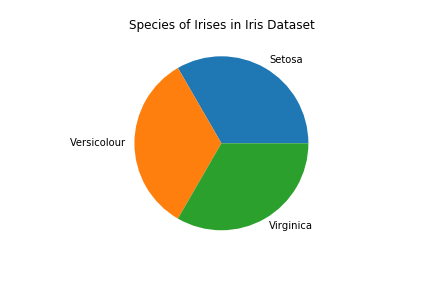
\includegraphics[width=\textwidth]{intro/iris_pie}
  	\caption{Relative amounts of each Iris species in the scikit-learn dataset\cite{scikit-learn}.}
  	\label{fig:iris_pie}
\end{figure}

\subsubsection{Bertin's Retinal Variables}
\begin{figure}
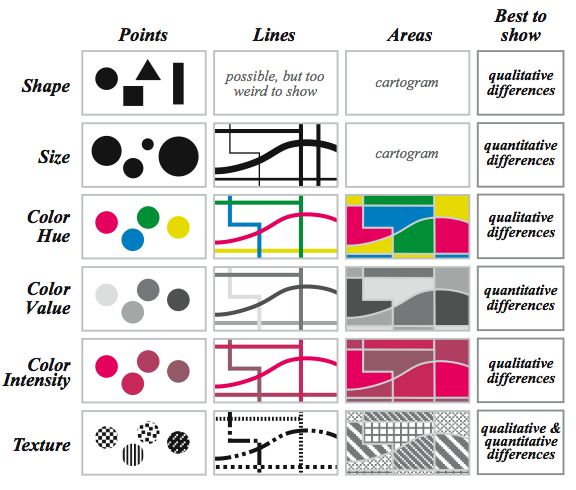
\includegraphics[width=1\textwidth]{intro/retinal_variables.png}
\caption{Bertin's retinal variables are a codification of how position, size, shape, color and texture can be used to illustrate variations in the components of a visualization. This tabular form of Bertin's retinal variables is from Understanding Graphics \cite{_information_????} reproduced from Making Maps: A Visual Guide to Map Design for GIS \cite{krygier_making_2005}}
\label{fig:retinal_variables}
\end{figure}

In figure~\ref{fig:iris_pie}, the invariant is the count of species and the components are the species themselves. In other words, the invariant is the value or calculation being visualized, and the components are usually the values on the axis and any variable encoded by what Bertin terms a retinal variable \cite{bertin_semiology_2011,krygier_making_2005}, which are the position, size, shape, color, and texture of the points, lines, or polygons in any visualization. As shown in figure~\ref{fig:retinal_variables}, Bertin recommends that quantative components be represented by retinal variables that change quantatively and that categorical components be represented by retinal variables that vary qualitatively. The small number of retinal variables suggests that visualizations are somewhat limited in how many components can be shown on any one graph.

\subsubsection{Munzner's data semantics}

\begin{figure}
 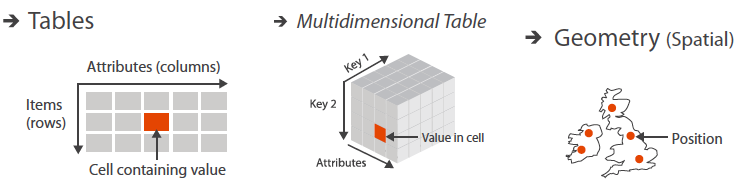
\includegraphics[width=\textwidth]{intro/munzner_datatypes}
\caption{Keys are unique lookup values used to find individual values in the dataset. Image modified from a diagram from Munzner's website \cite{_visualization_????}}
\label{fig:munzner_datatypes}
\end{figure}


A special class of data variables are those that provide situational information about an observational measurement, such as the time and place the observation was recorded. Tamara Munzner provides a classification system for thinking about the semantics of a variable \cite{munzner_what_2014}:
\begin{description}
\item[value] measurement of interest 
\item[key] uniqe index to look up value
\end{description}

\begin{table}
\begin{center}
\begin{tabular}{ l c r }
  Munzner & Statistics & Data Warehousing \\
  \hline
  key & independent attribute & dimension \\
  value & dependent attribute & measurement\\
\end{tabular}
\caption{Munzner's key, value designations are roughly analogous to independent and dependent semantics in statistics and what are commonly termed dimensions and measurements in the computer science community.}
\label{table:munzner_semantics}
\end{center}
\end{table}

As displayed in table~\ref{table:munzner_semantics}, keys and values are analogous to terms used within the statistics and data communities; the advantage of using keys and values is that they strictly refer to the real world semantics of the data\cite{munzner_what_2014}. Figure~\ref{fig:munzner_datatypes} illustrates how these keys are used to look up variables in a dataset. In a table or a database, it would be the primary key for a row, and in a map it could be an address or geopgraphic coordinates. In a multidimensional table, it could be a unique set of attributes-such as a timestamp, latitude, and longitude-associated with each measurment. 

Expanding on Munzner's key and value semantics, in many datasets the keys are discrete variables like time or geophysical location that are sampled from a continous curve, surface, or field. While these observations are discrete samples from the continous space, often the continuinous (functional) characteristic\cite{ramsay_functional_2006,muller_functional_2006} of the observational space is what is of interest.

\subsubsection{Conditional Probability}
\begin{figure}
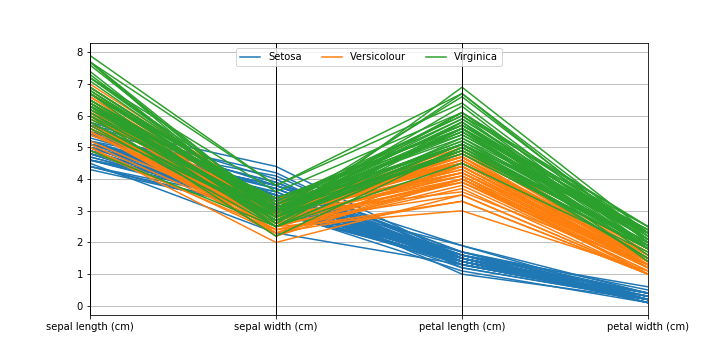
\includegraphics[width=\textwidth]{intro/iris_parallel}
\caption{The parallel coordinates plot (PCP) of the Iris dataset shows the pairwise relationship between adjacent variables, for example sepal length and sepal width. The PCP plot can be used as proxy for illustrating conditional probability because it shows how the quantitative measurements distribute amongst the species. This is is seen both in the relative widths of each band of color and in the similarities in shape of the orange and green (Iris Versicolour and Iris Virginica) bands and the consistent downward trend amongst the blue (Iris Setosa) bands.}
\label{fig:iris_parallel}
\end{figure}

While the Iris dataset does not have any variables that seem to traditionally fit into the model of keys-as it has no time or space variables-an analogous look-up task for the Iris dataset is to filter on a component and then look at the probability distributions of the other variables in relation tp that key. In effect this treats all variables as potential keys into distributions of the other variables. In the parallel coordinates plot (PCP)\cite{claessen_flexible_2011,_nist/sematech_????,inselberg_plane_1985, wegman_hyperdimensional_1990} in figure~\ref{fig:iris_parallel}, each line is an observation in the dataset, and each color maps to a species of Iris. The color coding then allows for this visualization to be used to show how the four quantative variables (sepal length, sepal width, petal length, and petal width) distribute within each variable. 

The visualization then becomes a way of visualizing the conditional probability of A given B:
\begin{equation}
P(A\mid B) = \frac{P(A \cap B}{P(B)} 
\end{equation}

wherein A is the observation vector $\left< \text{sepal length, sepal width, petal length, petal width} \right>$ and B in turn takes on each species of petal. The locations of the color and width of the colored band act as proxies for the distribution of each quantitative variable and the overall observation vector. 

\subsubsection{Conditional Dependency}
\begin{figure}
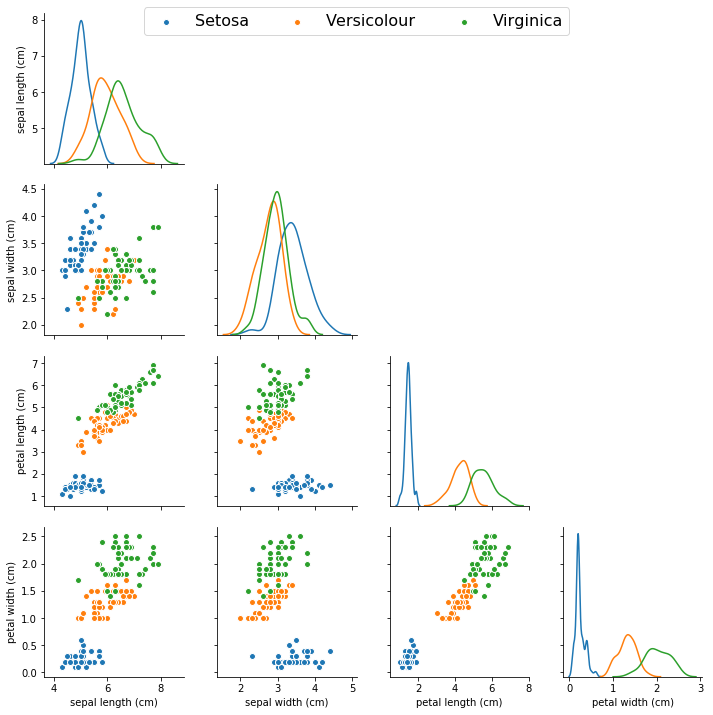
\includegraphics[width=\textwidth]{intro/iris_observations.png}
\caption{The diagonal of the scatter matrix shows the distribution of each variable relative to the species type. This can be used to illustrate the conditional probability of each variable relative to a type of species. The scatter matrix plot shows every set of pairwise relationships in the dataset, color code by Iris species. Because the scatter matrix shows the co-occurance of two variables and is encoded with information about a third variable, it works well was a tool to explore a potential conditional dependency amongst the variables.}
\label{fig:iris_observations}
\end{figure}

As exemplified by the scatter matrix\cite{elmqvist_rolling_2008,l._wilkinson_high-dimensional_2006} in figure~\ref{fig:iris_observations}, there are a number of visualization techniques that can be used to explore conditional dependencies, but these methods are limited to datasets where the observations are discrete. There are visualization techniques for understanding the probability distributions of functional observations that could potentially be leveraged in conjunction with these methods to develop methods for visualizing conditional dependencies in a functional space.


\begin{figure}
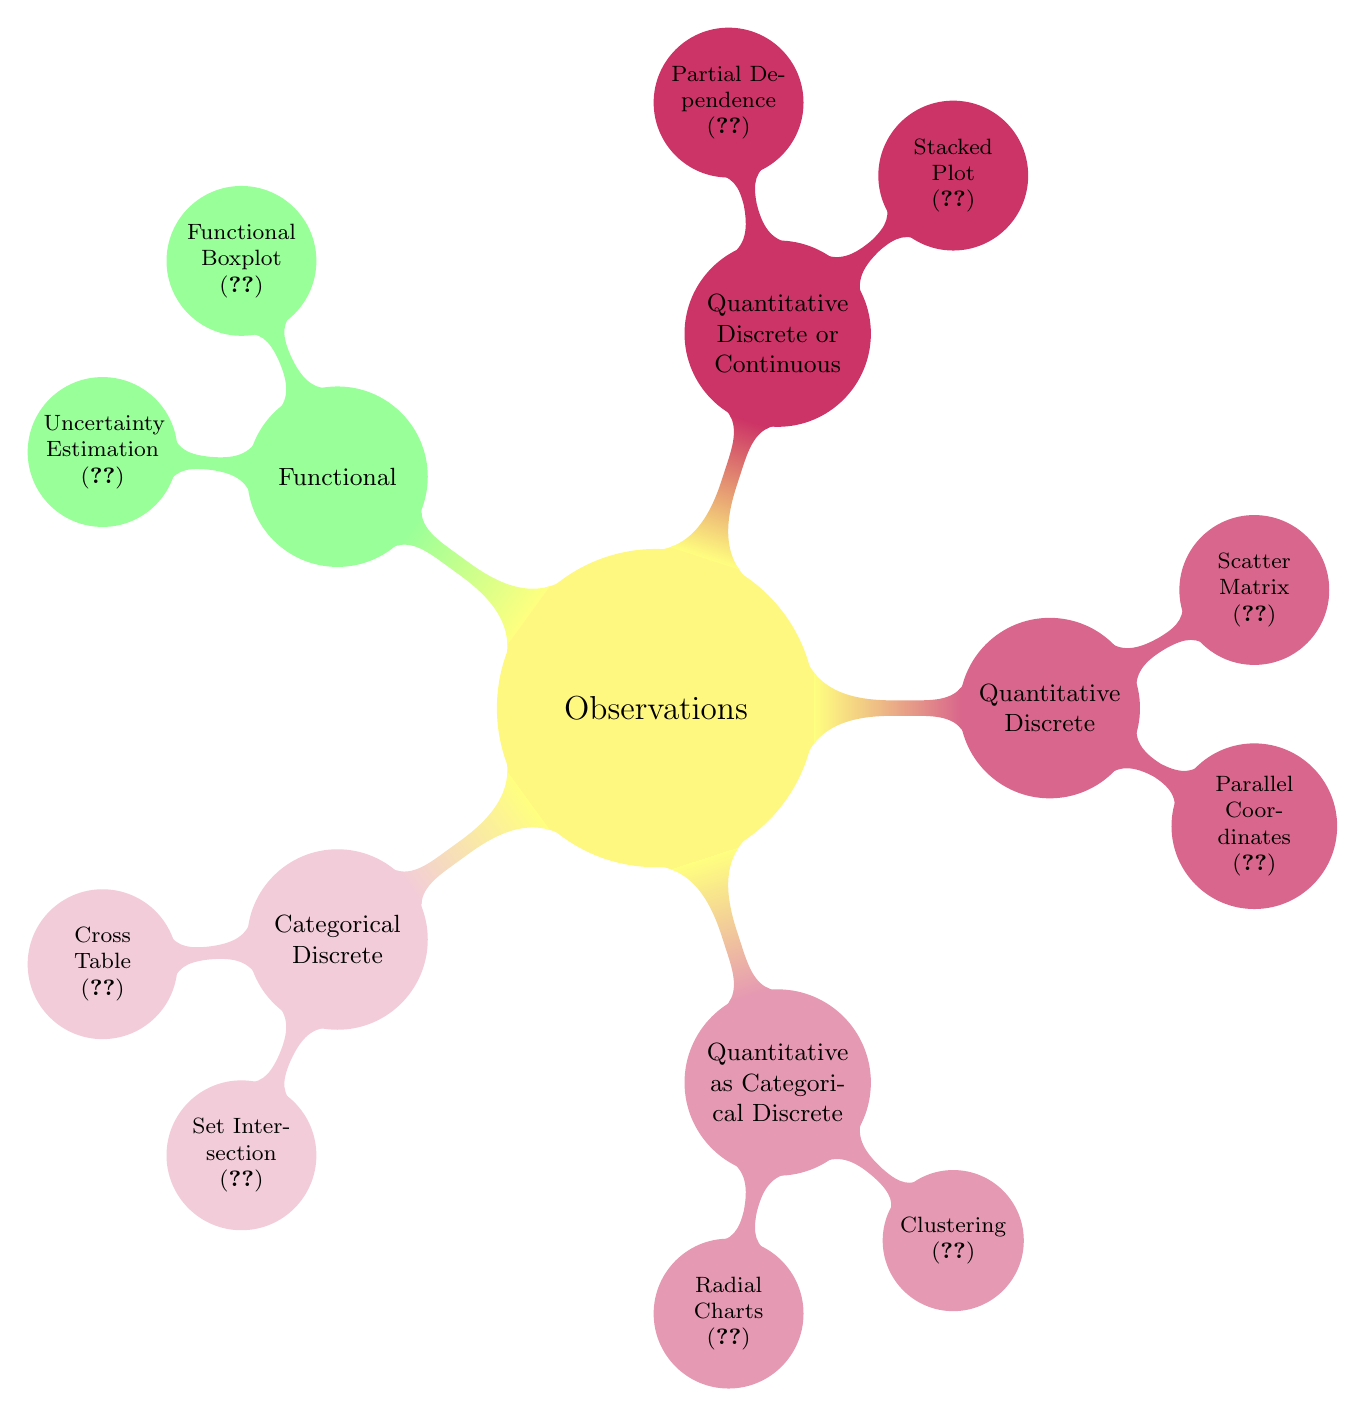
\begin{tikzpicture}[mindmap, grow cyclic, every node/.style=concept, concept color=yellow!50, 
    level 1/.append style={level distance=5cm,sibling angle=72},
    level 2/.append style={level distance=3cm,sibling angle=60},]
    
\node{Observations}
    child[concept color=purple!20]  {node {Categorical Discrete}
            child {node{Cross Table\\(\ref{sec:crosstab})}}
            child {node{Set Intersection\\(\ref{sec:setintersection})}}
            }
    child[concept color=purple!40]  {node {Quantitative as Categorical Discrete}
            child {node{Radial Charts\\(\ref{sec:radial})}}
            child {node{Clustering\\(\ref{sec:cluster})}}
        }
    child[concept color=purple!60]  {node {Quantitative Discrete}
                    child {node{Parallel Coordinates\\(\ref{sec:pcp})}}
                    child {node{Scatter Matrix\\(\ref{sec:condep})}}
        }
    child[concept color=purple!80] {node {Quantitative Discrete or Continuous}
                    child {node {Stacked Plot\\(\ref{sec:stacked})}}
                    child {node{Partial Dependence\\(\ref{sec:pdp})}}
        }
    child[concept color=green!40]  { node {Functional}
        child {node{Functional Boxplot\\(\ref{sec:boxplots})}}
        child {node{Uncertainty Estimation\\(\ref{sec:uncertainty})}}
    }
;
\end{tikzpicture}
\caption{The papers in this survey are organized by the type of observation and then by the type of measurements that makes up the observation.}
\label{fig:papermap}
\end{figure}

 This survey organizes the methods for exploring conditional dependency by observation type and data semantics, as shown in figure~\ref{fig:papermap}. In the functional space, the focus is on visualizing distributions because that is a necessary component of exploring conditional dependencies. 





\section{Discrete Observations}
\subfile{sections/catset}
\subfile{sections/radclust}
\subfile{sections/pairwise}
\section{Continuous Observations}
\subfile{sections/quantKquantV}

\section{Conclusion}
\label{sec:conclusion}

From climate models to Internet advertisement, a lot of modern datasets are very large and often structurally complex. And the questions being asked of these datasets are increasingly probabilistic-what is the distribution of observations, under what events do observations occur, and are there events that have to happen? The latter question is the one explored in conditional dependency visualizations. As explored in this paper, there are many techniques for exploring these dependencies in the discrete observation space, and there is a lot of work being done to understand distributions in the latter space. There is a space for future work that would leverage both to develop conditional dependency visualizations for functional datasets. 

\printbibliography
\end{document}
